\chapter{Solution design}
In this chapter, we would like to explain the thinking process before and during the implementation of the back-end application. We explain the problems that we have to solve in the implementation part. We reveal the possible ways to solve the problems and describe how we solved them in the end.

\section{Authentication}
In our application, we had to deal with authentication for customers and employees. There are many ways how users can be authenticated using the REST API. We ended up with token authentication - in each request frontend applications must set the Authorization header with the authentication token as a value. Front-end application can retrieve the token in exchange for correct credentials.

Another part of the authentication we have to consider is at least the basic security during the manipulation with authentication data and flawless verification token sending.

\subsubsection{Token authentication details}

We decided to implement the token authentication on our own, using only Rails helpers for generating and verifying secure tokens. As you can see in \ref{auth-token-scheme}, the token is generated during the login action and then returned in a body response. In order to be considered authenticated, all the following requests must have this token present in the headers .

\begin{figure}[h]\centering
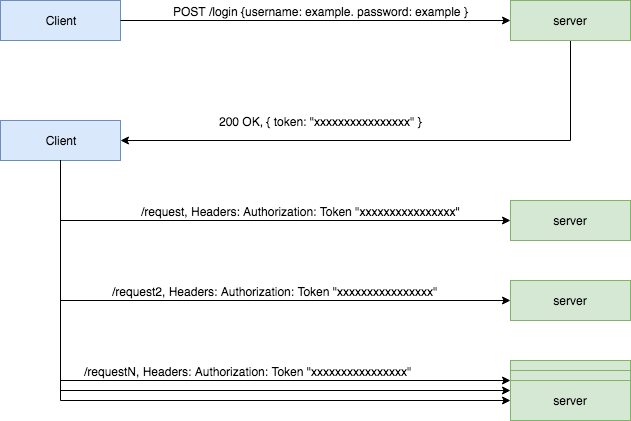
\includegraphics[width=\textwidth]{auth/Auth.png} 
\caption{Auth token scheme}\label{auth-token-scheme}
\end{figure}

Our application store just one token per user. That implies the user can be logged in from one device at a time only. Having more valid token for users would let into several problems with the invalidation in case of logging out.

In Ruby on Rails there exists a very good gem for authentication called \textit{devise\_token\_auth} \footnote{\url{https://github.com/lynndylanhurley/devise\_token\_auth}}. This library is always the first choice if a Ruby on Rails developer implements the authentication system. However, we decided not to use it in the end. In the following paragraphs, we explain why.

The first reason for not using the gem is that it uses an email address as the default authentication field. For the customers we wanted to use the telephone number as the main identifier, which would lead us to rewrite most of the library's controllers and models anyway.

The second reason was the complexity of the whole authentication process which the gem forced us to use. This library would provide a more secure but also much more complex way of authenticating in our project. Once the client gets the token from the login endpoint, a new token is generated and returned with each following request. Using this approach arises the batch request problem. Imagine that the front-end application sends three requests to the server at once. Of course that all of the three requests must have the same authentication token - the front-end doesn't have the new token until the response. This implies the server must accept all of those three requests as authenticated. Besides that the back-end and front-end must agree on which of the responses has the new correct auth token - responses don't have to come in order in which they were sent. This complicated process was implemented in the back-end gem and couldn't be easily changed. The front-end part of the library seemed to be implemented, but after the three weeks of trying and founding several bugs in the library - without even successful login - we gave up using it.

This implies that if we had wanted to use the gem on backend we would have to understand the whole gem auth process in detail and specify it for the front-end. Front-end would then have to write the whole complicated solution from scratch. 

We came to the conclusion that the complexity which would bring this library to our application is not worth the better security and stability we would gain from using it. Forcing the HTTPS protocol for the communication between the server and front-end applications makes the token theft more difficult in this case. Also, the only really sensitive accounts for identity theft are the employees' ones. Furtunatelly we are in personal contact with them regularly, so we get to know about the potential account misuse or hack quickly. Also, we can provide a more secure and better solution later.

\subsubsection{Basic security}
	As we mentioned in the last paragraphs, our token solution is not perfect from the security perspective. Besides the token (which could be easily rewritten more securely in the future ) we tried not to take the security of our application lightly.
	
	First of all, we don't store passwords in plaintext. We use Rails integrated feature \textit{has\_secure\_password}\footnote{\url{https://api.rubyonrails.org/classes/ActiveModel/SecurePassword/ClassMethods.html}}, which uses BCrypt hash function.
	
	As a result of using the Ruby on Rails tools correctly we also excerpt the passwords from all of the application logs, and we are not vulnerable to SQL Injection\footnote{\url{https://en.wikipedia.org/wiki/SQL\_injection}} attack.

\subsubsection{Verification tokens sending process}
	We send the verification tokens via emails and SMS during the account manipulations. These actions are not instant (API request, SMTP request) and in Rails we can easily create asynchronous workers. We decided to have these functions handled via Sidekiq workers. In exchange for some time spent on the configuration we don't block web server threads during account creation/recovery token sending and we also have the ability of resending the messages automatically in case of the third party or network failure.

\section{Secrets}
	In our application, we have to keep several API tokens, database passwords, and other sensitive information. We store those secrets in files which are not tracked in the version control system. Those files are then loaded by the Docker, which sets them as environment variables. From these variables we read this sensitive information in the whole application.  

\section{Authorization}
Almost every endpoint has its own rules of who and in what circumstances can do this action. There are two main groups of users - employees and customers. Employees are then divided into three groups - administrators, drivers and dispatchers. There are just two types of customers - registered and unregistered. Each visitor is one of those types.

In each request we solve the condition whether the current user is able to execute the requested action or not. Having all these conditions directly in controllers would make the controllers difficult to read. Also, these conditions could (and did) have changed during the development iterations. This led us to have the authorization conditions separated in the different part of the application.

We wanted to avoid reinventing the wheel so we have chosen to use the \textit{Pundit} \footnote{\url{https://github.com/varvet/pundit}} gem. 

Another option came across during the research was the \textit{Cancancan} \footnote{\url{https://github.com/CanCanCommunity/cancancan}} gem. They both have a long maintenance history, they are actively developed in the time of writing and they satisfy all of our requirements for the authorization. \textit{Cancancan} is better suited for the applications with complicated views because it provides more helpers for checking the authorization in them. Its architecture is also more general thus it is better optimized for more complicated permission management. That results in slightly more complex permission definitions. On the other side, the \textit{Pundit} is a more light-weight solution with very simple architecture and permissions definition files. Because our permissions are not complicated very much and we wanted to have them written as simply as possible, this was the main reason why we chose \textit{Pundit} over \textit{Cancancan}.
.

 \section{Pagination}
 As the data grows some of the requests (e.g. order index) would return thousands of items. This would be a huge waste of resources, so we have to limit the count of returned items per request and enable pagination. For such purpose, there exists a gem \textit{Kaminari}\footnote{\url{https://github.com/kaminari/kaminari}} which adds methods for quick filtering and retrieving data in our models. We just define pagination request parameters and pass them to this library. Also thanks to the global configuration we can limit the maximum number of results per page.

\section{Rendering views}
	Even though whole view layer is just about displaying simple JSON objects, we use whole separated view layer from the Ruby on Rails framework with the help of \textit{Jbuilder} gem\footnote{\url{https://github.com/rails/jbuilder}}.
	
	At the beginning of the implementation we thought that we don't have to have the view part separated from the controller. For simple entities such as vehicles, it was sufficient. When we started to have more complicated requirements for the views - such as displaying different attributes for different user roles, most of the controller's code was the view logic which obscured the controllers.
	
	\textit{Jbuilder} allows us to have the view code separated from the controllers and gives us the simple syntax to extract desired fields and parts from our variables to JSON.
\section{Images}
	Our employees and vehicles contain images. We had to figure out how to get the image from the frontend application via the REST API to our backend application. 
	
	We ended up with two options on how to implement it. First is the multipart HTML requests\footnote{\url{https://tools.ietf.org/html/rfc7578}}. The second option is to encode the image into Base64 on frontend and then send it in a request body as JSON field. This field is then decoded on the server side and saved.
	
	We decided to go with the second option in the end. On both front-end and back-end, we have the libraries for processing images this way so the implementation was easier on both sides. The downside of this solution is that we can not transfer as much data this way as in the multipart request option. However, we have only one image for each employee and vehicle thus this solution is sufficient.
	
	For the back-end side we decided to use the \textit{Carrierwave::Base64} \footnote{\url{https://github.com/y9v/carrierwave-base64}} gem. Besides the out-of-the-box Base64 encoding of a specified attribute which we need, it provides the simple API for the storage settings such as file names. Also in case of switching our storage to some cloud storage provider such as the S3 by Amazon\footnote{\url{https://aws.amazon.com/s3/}} in the future, it would be just the matter of changing few lines in the configuration. 

\section{Customers}
Using the email address as the main authentication field is kind of standard. We came to the conclusion that we should use as our identifier telephone number. Despite the standard and the consequence of this decision - lack of any easy-to-use library for the authentication in Rails. Reasons which led us to this decision:
\begin{itemize}
	\item In case of emergency during the order process we must be able to contact the customer immediately, so we need the customer's phone anyway.
	\item Customers are going to register and order taxis from their phones most of the time. 
	\item Not everyone has direct access to the mailbox from its the phone - unlike the SMS which has every phone built-in. 
\end{itemize}
\subsection{Create and confirm}
Besides the authentication problems described in before, we have to deal with the telephone verification.

We decided to use verification via the SMS code.

A registered telephone number must be verified.  Before the customers can do so, they must go through telephone number confirmation process as follows: Customers receive SMS with a registration token. This token is valid for 5 minutes, and the customer can ask for resending.  Resending will invalidate the last token, generate a new one and send it. Confirm is made with provided token and the telephone number.

Based on the requirements we decided to split these functions into three API endpoints - \textit{create}, \textit{confirm} and \textit{resend\_confirmation}.
 
 \subsection{Password recovery}
 The whole password recovery procedure is similar to the create account one.
 Based on specification we split the password recovery feature into two API endpoints - \textit{password\_recovery} and \textit{reset\_password\_by\_token}. 
 
 Calling the first endpoint - password recovery - sends in exchange for the telephone number SMS to that telephone number with password recovery token. Then the customer can send a request with this token, his telephone number and a new password - which if all the conditions are satisfied - will be set. 
 
 The token consists of 4 numbers and is valid for 5 minutes. These parameters we just picked are similar to the other services on the internet. Of course we are able to change them later easily if we discover that it's not suitable.
 
 We have noticed that the \textit{password\_recovery} endpoint must - except the bad request format - always return the success status. Especially we can not let the client know that the account with such telephone number was not found and neither that the SMS was not sent successfully. If we would return an error code in such a situation, an attacker could get all the telephone numbers of all of our customers this way.
 
 We are aware that the SMS may not be the most secure way of verifying users\footnote{\url{https://www.cnet.com/how-to/why-you-are-at-risk-if-you-use-sms-for-two-step-verification}} but we think that at our scale, potential losses for stolen customer's account wouldn't be crucial - there is no credit system or something valuable on the account. The worst case scenario is that the attacker creates an order on behalf of the victim and thus that order will be a fraud. However, the fraud orders occur a few times a week anyway.
 
 \subsection{Favourite places}
 We decided to have an endpoint with four parameters, which will return the list of N recommended places ordered from the most to the least appropriate.
 
 The first parameter is the maximum number of places we would like to receive, second is customer id for whom we want to have recommendations for, third is the location and the last \textit{start} parameter acquires one of the following values:
 \begin{itemize}
 	\item true = we want recommendations for pick-up places, the provided location is the customer's current location
 	\item false = we want recommendations for drop-off locations, the provided location is the pick-up location
 \end{itemize}
 
 Our first problem to solve is how to handle the locations from the request. We suppose that the location which goes to our API is directly from the customer's telephone sensors, thus there's nothing like Example's restaurant official coordinates, which would client sent to us whenever he wants a taxi from that restaurant. On the other hand, we would like to group all these locations near the Example restaurant into one place, so we can later recommend it just once. On the other side, the tolerance must be small enough to not to join together two different places. We thought about using some kind of modified clustering algorithm but we ended up with a conclusion that this would be an overkill in our case . We came to a conclusion that for our use case is having some distance tolerance constant defined enough. Then all of the places within this distance are considered as one place. We set this constant to 50 meters because it seemed like a good compromise between the inaccurate low-end GPS sensors precision and the distance between two different places. Of course, we are able to change this constant in the future in case we discover that it is too small or big.
 
 The second problem was how to filter and return the list of places fast. For each user, we have an index of visited places with the information based on which our algorithm recommends. In this index we have the following information about each place:
 \begin{itemize}
 	\item coordinates
 	\item list of items containing for each place occurrence in orders:
 	\begin{itemize}
 		\item a decimal number from 0 to 1 which says, how long ago was order with this place placed. 1 has user's last order and 0 has user's furthermost order.
 		\item time-stamp when was the order created
 		\item start = whether was the place in the order used as a start or finish
 	\end{itemize}
 	\item list of corresponding places (drop-off for pick-up and vice versa)
 \end{itemize}
For the given parameters in a request, we go through the index place by place and count its weight as a sum of the weights where the place occurs multiplied by a constant if start/finish fits the desired index direction. The index is also prepared for the places recommendations based on the order time (e.g. in the evening we go to the pub, in the morning to work). We decided to limit the recommendation index for last 1000 orders for each user.

In our research we haven't found any ready-made solution for this problem, so we decided to come up with our own solution. We are aware of the fact that it could be more effective and recommendation could be more sophisticated. However, we came to this algorithm during the development and it satisfied all our desired requirements so we kept it.

\section {Order scheduler}

The goal of order scheduler in our application is to distribute the new orders between the drivers. Besides that, the system accepts other actions for order manipulation. These actions are then reflected to the corresponding driver's queue and to all of the orders affected by such actions.

First of all, we have to deal with the distance calculation. All we know about the new order are just the pick-up and the drop-off location coordinates. Based on this information we have to calculate the distance and the duration of the order. Each order consists of the two parts we have to calculate. The first part is from the pick-up location to the drop-off location. This part is fixed for each of the orders. The second part is the route between the driver and the pick-up location. This part differs for each of the drivers. For the distance and duration computation, we decided to use the \textit{Google Maps Distance Matrix API} \footnote{\url{https://developers.google.com/maps/documentation/distance-matrix/intro}} which allows us to get the distances between all the drivers and the order pick-up location in a single request. Also choosing this API allows us to use the existing Ruby Gem \textit{googlemaps-services}\footnote{\url{https://github.com/amrfaissal/googlemaps-services}}. This library provides the Ruby interface for the communication with that API. This API can also calculate the distance and duration with respect to the current traffic.

The second problem we are facing are the scheduled orders. Arriving at the pick-up location on time is the priority number one. Because of the business requirements scheduler does not assign these orders to a driver automatically but the dispatchers do that manually. This implies that in our system could appear order collisions which must the system handle correctly. We have to take in to account the high cost of each route calculation too.

Based on the specification we decided that order scheduler system accepts these actions:
\begin{itemize}
	\item Add
	\item Change arrive time
	\item Cancel
	\item Change driver
\end{itemize}


In the following subsections we describe possible situations that can occur in each of these actions, how the planning system should handle them and how it should respond to them. We display the situations using the diagrams described in the legend \ref{order-planning-legend}.

\begin{figure}[h]\centering
	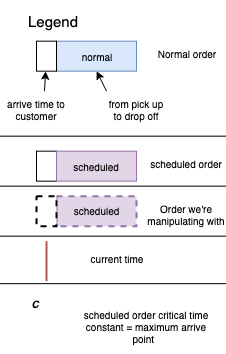
\includegraphics[scale=0.7]{orders/legend.png}
	\caption{Order planning scheme legend}\label{order-planning-legend}
\end{figure} 



\subsection{Add order}
We distinguish two main categories of added orders - scheduled order and normal (not scheduled) order. At first, we define who can be assigned to the order, then we define how to do it.

Order can be assigned to either any of the available drivers or to a specific driver. By available driver, we mean the driver who is on shift and is not in the pause state. From this set of drivers, we choose the driver who will be assigned to the order. In case that there is no driver suitable scheduler raises an error.

As mentioned before, the scheduler must ensure that if the scheduled order is assigned to the driver, the driver is able to get there right on a specified pick-up time. This reveals the problem - how to calculate the time when the driver should start arriving towards the customer (\textit{start\_est time})? To calculate it we must calculate the arriving duration between the driver location and the pick-up location. The problem is that the expected driver location changes with each assigned order.

First naive solution led us to count the start time when we add the order to the queue. In this point we know the finish location of order before, so we could count arrive time from that point. The problem is that the scheduled order can (and probably will) start a week or two from now. In order to persist the calculated start time, we have two options. First one is to forbid adding new orders before the scheduled order. This is obviously unacceptable. The second one is that during the insertion of some other order in between the last order in the queue and our scheduled order, we calculate two start times - the newly inserted one and the scheduled one \ref{scheduled_naive_arrive_counting}. 

\begin{figure}[h]\centering
	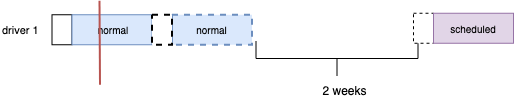
\includegraphics[scale=0.7	]{orders/scheduled_naive_arrive_counting.png}
	\caption{Scheduled order - naive arrive time calculating approach} 
	\label{scheduled_naive_arrive_counting}
\end{figure} 

Each route calculation is expensive and this naive approach doubles the costs of each processed order for the drivers who have some scheduled order in their queue. Because these orders with two weeks ahead pick-up time are the most common in our taxi company we want to avoid this extra cost. 

We observed that there must be some point when the start time of the scheduled order must be calculated. If we calculate it too early, we raise the costs per order. If we calculate it too late, the driver may not be able to get to the pick-up location on time. 

Our solution combines these two approaches. Based on that observation we define the critical time constant \textit{C}. Value of this constant is equal to the maximal arrive time to any location operated by the taxi company. 

In our scheduling system then holds this fact: For each scheduled order in a queue, which has pick-up time less than \textit{C} from the current time or the finish time of order before, it holds that its start time is calculated. This time is then updated with each relevant change in the queue. If the distance between two orders in a queue is larger than \textit{C} the start time is equal to pick-up time.

The whole process of calculating the arrival and start time led us to split the problem of adding the order to queue into seven parts:
\begin{itemize}
	\item Normal order - calculating the arrival time
	\item Normal order - selecting the driver
	\item Scheduled order - calculating the start time
	\item Scheduled order combined with other scheduled order
	\item Scheduled order combined with normal order
	\item Normal order combined with scheduled order
	\item Scheduled order - scheduling at critical time callback 
\end{itemize}

	\subsubsection{Normal order - calculating the arrival time}
	
	First, we focus on how to calculate the normal order's arrival time. As we can see in \ref{order-process-normal-order-counting-arrive} there are three states in which the queue can be.
	
	As in the situation \textit{1a)} if the last order in queue is a normal order, calculate the arrival time as the sum of the last order finish time and the duration between the orders' finish and start location.
	
	In case that the queue is empty as in \textit{1b)} calculate the arrival time as a current time plus the driver's average response time to order plus the duration between the last driver's known location and order pick-up place.
	
	Third possible situation \textit{1c)} occurs when there is an ongoing scheduled order. Then the arrival time is calculated as the time between finish location of that order and start of the new order.
	
	
		\begin{figure}[h]\centering
			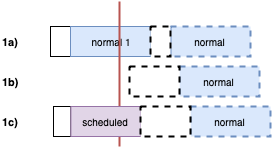
\includegraphics[scale=0.7	]{orders/add-1.png}
			\caption{Normal order - calculating the arrival time} 
			\label{order-process-normal-order-counting-arrive}
		\end{figure} 
	
	\subsubsection{Normal order - selecting the driver}
	
		As described in specification normal order must be always assigned to the driver who can pick up the customer first. This rule demonstrates the example  \ref{order-process-normal-order-selecting-driver}. The order will be assigned to the \textit{driver 1} even though the \textit{driver 2} is available first.
		
			\begin{figure}[h]\centering
				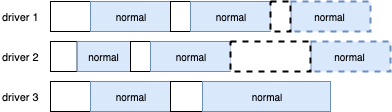
\includegraphics[scale=0.7	]{orders/add-2.png}
				\caption{Normal order - counting arrive} 
				\label{order-process-normal-order-selecting-driver}
			\end{figure} 
		
	\subsubsection{Scheduled order - calculating the start time}
		If we add a scheduled order to the driver's queue in which there is no other order within the critical time constant, we do not calculate the arriving duration of that order\ref{order-process-scheduled-order-counting-arrive-time}. We are allowed to do so because the critical time constant \textit{C} ensures that even if the queue stayed in the same state, the arriving duration between the last driver's location to the order start will be less than \textit{C}.
		
		\begin{figure}[h]\centering
			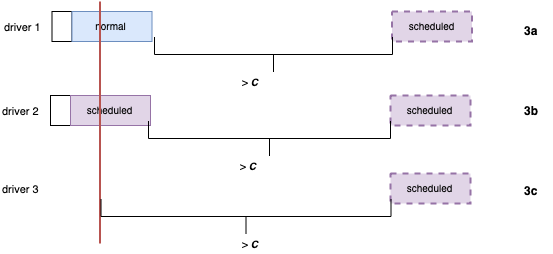
\includegraphics[scale=0.7	]{orders/add-3.png}
			\caption{Scheduled order - counting arrive time} 
			\label{order-process-scheduled-order-counting-arrive-time}
		\end{figure} 
	
	
	\subsubsection{Scheduled order - combined with other scheduled order}
			In case that the scheduled order has other scheduled order within the \textit{C} from the calculated pick-up or finish time, we have to calculate corresponding order start times \ref{order-process-scheduled-order-combined-with-scheduled}. 
			After the calculation, we may encounter the orders collision. In such a case, the order cannot be added to the queue and the order scheduler must throw an error. 
			
			\begin{figure}[h]\centering
				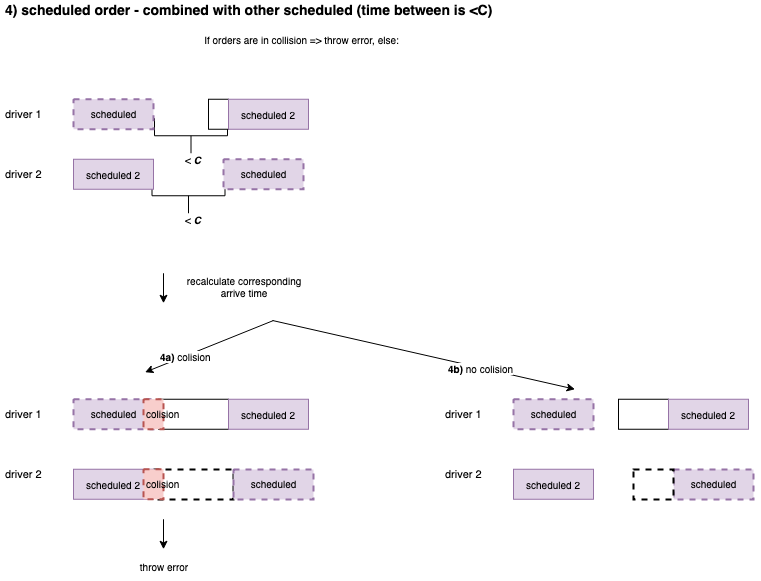
\includegraphics[scale=0.6	]{orders/add-4.png}
				\caption{Scheduled order - combined with other scheduled} 
				\label{order-process-scheduled-order-combined-with-scheduled}
			\end{figure} 
		
	\subsubsection{Scheduled order combined with normal order}
		When the expected finish time of last normal order in queue is within the \textit{C} from the inserted order's scheduled pick-up time, we must calculate the arriving duration. In case that the the scheduled order is in collision with some normal order, scheduler must throw an error \ref{order-process-scheduled-order-combined-with-normal}.
		 
		\begin{figure}[h]\centering
			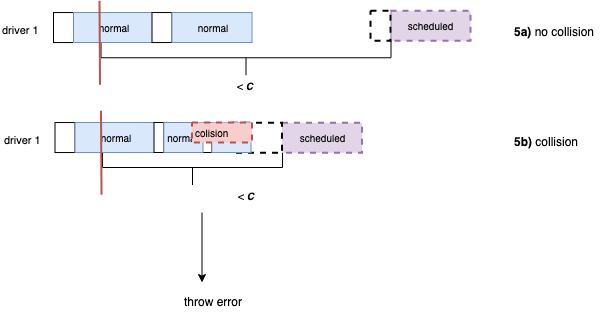
\includegraphics[scale=0.6	]{orders/add-5.png}
			\caption{Scheduled order - combined with normal order} 
			\label{order-process-scheduled-order-combined-with-normal}
		\end{figure} 
	
			
	\subsubsection{Normal order combined with scheduled order}
	Adding a new normal order to queue could break the fact that each of the scheduled orders in our system has the arriving duration calculated if the pick-up time is at least \textit{C} from the finish time of order before it.
	
	If this situation occurs, we must recalculate the arriving time of the scheduled order after it -  accordingly with respect to the new finish location. This change can lead to a collision. In case we encounter the collision, we start the process of adding the order again. In this second try we consider the scheduled order as a last order in this queue so in case of choosing this queue again, the normal order will be inserted after it. Also the arrive time of the colliding scheduled order must be set back to the original value. 
	 \ref{order-process-normal-order-combined-with-scheduled}.
	
	\begin{figure}[h]\centering
		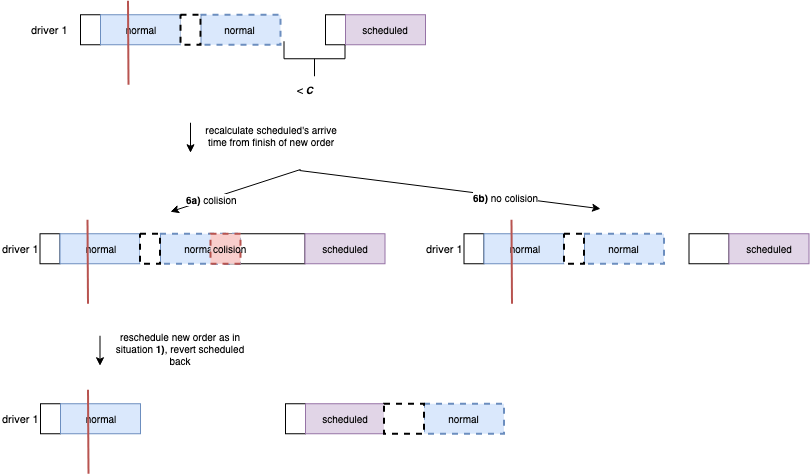
\includegraphics[scale=0.5	]{orders/add-6.png}
		\caption{Normal order - combined with scheduled order} 
		\label{order-process-normal-order-combined-with-scheduled}
	\end{figure} 

	\subsubsection{Scheduled order - scheduling at critical time callback}
	As we know, scheduled orders do not have the arriving duration calculated only when there is no order in queue with a finish time within the \textit{C} from the pick-up time or the pick-up time is not within the C from the current time. In previous cases we described all the possible situations how can order be added before the scheduled order within the time constant. Last thing we have to cover is the situation when the current time exceeds a point from which is the the pick-up time of our order less than C.
	
	This situation we cover with a callback which is called exactly in that point. If in this point the order does not have the start time calculated, we calculate it from the last known driver's location and the order start location. 
	 \ref{order-process-scheduled-critical-time}.

	\begin{figure}[h]\centering
		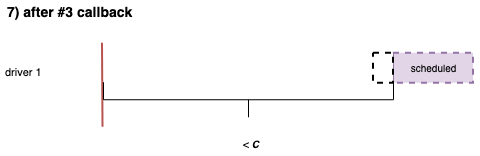
\includegraphics[scale=0.7]{orders/add-7.png}
		\caption{Scheduled order - critical time callback} 
		\label{order-process-scheduled-critical-time}
	\end{figure} 

\subsection{Change arrive time}
	Estimated order times can be manually changed by driver during the order. Average expected time change in such cases is within a few minutes. We can divide the change of time into two groups. In the first one the order will take longer after the change, in the second one the order will be shorter.
	
	\subsubsection{Longer order}
	When the order takes longer than it was expected to, we just take all the normal orders after it until the first scheduled one and we move their start times accordingly\ref{order-process-change_longer}.
	\begin{figure}[h]\centering
		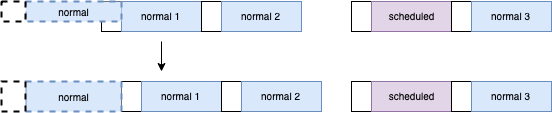
\includegraphics[scale=0.7]{orders/changing_arrive_time_longer.png}
		\caption{Change arrive time - longer order} 
		\label{order-process-change_longer}
	\end{figure} 

	During this change there can occur a collision with some scheduled order in queue. If the colliding order is normal order, we reschedule it the same way as we were adding it \ref{order-process-change_collision_normal}. 
	
	\begin{figure}[h]\centering
		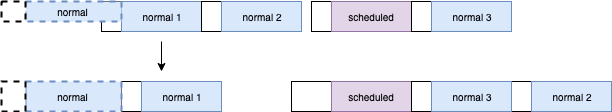
\includegraphics[scale=0.65]{orders/changing_arrive_time_longer_normal_collision.png}
		\caption{Change arrive time - longer order - collision of normal and scheduled order} 
		\label{order-process-change_collision_normal}
	\end{figure} 

	If the collision causes other scheduled or an ongoing order, we must shift the start of the scheduled order \ref{order-process-change_collision_scheduled}.
	
	\begin{figure}[h]\centering
		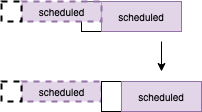
\includegraphics[scale=0.7]{orders/changing_arrive_time_longer_scheduled_collision.png}
		\caption{Change arrive time - longer order - collision of two scheduled orders} 
		\label{order-process-change_collision_scheduled}
	\end{figure} 
	
	
	\subsubsection{Shorter order}
		When the time change makes the order shorter, we just simply change the start time estimations accordingly for all of the normal orders after the changed one until the first scheduled order in queue.
		\ref{order-process-change-shorter}.
		
		\begin{figure}[h]\centering
			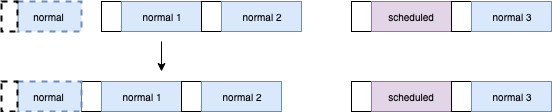
\includegraphics[scale=0.7]{orders/Shorter_order.png}
			\caption{Change arrive time - shorter order} 
			\label{order-process-change-shorter}
		\end{figure} 
	
\subsection{Cancel}
	When the order is cancelled, we must remove it from the driver's queue and reschedule each order after the cancelled order - except the scheduled one. By rescheduling we mean sequence of two actions - \textit{cancel} and \textit{add} \ref{order-process-cancel}.
	
	\begin{figure}[h]\centering
		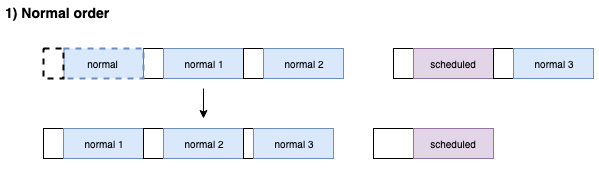
\includegraphics[scale=0.7]{orders/cancel.png}
		\caption{Cancel the order} 
		\label{order-process-cancel}
	\end{figure} 
	We suppose that the order cancel is rarely called, so we do not pressure on the route calculation optimization as much.

\subsection{Change driver}
Changing the driver should happen even less than cancelling the order. In such case it is sufficient just to call the \textit{cancel} action and \textit{add} action with the specified selected driver.
	 
	 
	 
\section {Orders}

	For our application it is critical to keep track of the order modification history. In case of unsuccessfully handled order we must be able to tell whether it was the scheduler failure or the mistake was caused by an employee or a customer. Also having the order time estimations history may help us in the future with improving the scheduling system. We have found the \textit{paper\_trail} gem\footnote{\url{https://github.com/paper-trail-gem/paper_trail}} which fulfils our needs and is easy to use and setup.
	
	
	Second problem we have to deal with in the orders was how to store the time information we are keeping the track of. In one half of the application we have to know and modify the time durations (arrive, picking up) and in the other half we have to know exact times (start, arrival to customer, finish). We have two options how to save such times. We can preserve timestamps for each event and the durations compute on demand. We decided for the second option - save the order start timestamp and the durations in seconds for the rest. Thanks to this approach we can easily manipulate the orders in scheduler.  Downside of this approach is that we can not easily filter and sort the orders based on those calculated time attributes.   
